\documentclass{if-beamer}
\usepackage{ctex}

\makeatletter
\let\@@magyar@captionfix\relax
\makeatother

\usefonttheme[onlymath]{serif}

% --------------------------------------------------- %
%                  Presentation info	              %
% --------------------------------------------------- %
\title[平衡态统计物理讨论班]{有了玻尔兹曼方程之后我们能做些什么}
\subtitle{基于玻尔兹曼方程的推导计算\&热寂说}
\author{钱思天}
\institute[PKU]{
  Peking University
}
\date{\today}

\subject{Presentation subject} % metadata

\graphicspath{{figuras/}}
% --------------------------------------------------- %
%                    Title + Schedule                 %
% --------------------------------------------------- %

\begin{document}

\begin{frame}
  \titlepage
\end{frame}

\begin{frame}{目录}
  \tableofcontents
\end{frame}

% --------------------------------------------------- %
%                      Presentation                   %
% --------------------------------------------------- %
\section{玻尔兹曼方程}
\begin{frame}{玻尔兹曼方程}
\begin{exampleblock}{玻尔兹曼方程}
\begin{equation*}
    \frac{\partial f}{\partial t}+\nabla_{\vec{r}} \cdot(f \vec{r})+\nabla_{\vec{v}} \cdot(f \dot{\vec{v}})=\int\left(f_{1}^{\prime} f^{\prime}-f_{1} f\right) d \vec{v}_{1} \Lambda d \Omega
\end{equation*}
\end{exampleblock}
\begin{columns}

\begin{column}{0.5\textwidth}
    
    \begin{block}{从玻尔兹曼方程出发我们可以……}
        \begin{description}
            \item [细致平衡条件:] 如何从玻尔兹曼方程到平衡态分布函数;
            \item [弛豫时间近似:]如何将玻尔兹曼方程的从微分积分方程进行化简;
            \item [H函数与熵:]H函数与熵是否存在一定的关系;
            \item [……]
        \end{description}  
    \end{block}

\end{column}

\begin{column}{0.5\textwidth}
\begin{alertblock}{注意}
    在推导玻尔兹曼方程时我们假设:
\begin{itemize}
    \item 假定是经典稀薄气体,分子力是短程的.
    \item 把分布函数的变化分成漂移项和碰撞项两部分,在计算
    漂移项时,不考虑分子之间的相互作用和碰撞;而在计算碰撞项
    时,也完全不考虑分子在外力作用下的运动.
    \item 只考虑二体碰撞.
    \item 忽略分子的内部结构.
    \item 在计算元碰撞与元反碰撞数时,引入分子混沌性假设.
\end{itemize}
    
\end{alertblock}
    
\end{column}




\end{columns}
\end{frame}
\subsection{细致平衡条件与平衡分布}
\begin{frame}{细致平衡条件与平衡分布}
    系统的平衡态由细致平衡条件所保证。
    因此,从细致平衡条件出发,我们应当能够推导出平衡态分布函数。并且这个分布函数必须是唯一的。

        \begin{block}{细致平衡条件}
            \begin{equation*}
                \begin{aligned}
                    f_1f_2&=f_1'f_2'\\
                    \ln{f_1}+\ln{f_2}&=\ln{f_1'}+\ln{f_2'}
                \end{aligned}
            \end{equation*}
        \end{block}
        \begin{block}{}
            取对数后的细致平衡条件有着碰撞守恒的性质,而碰撞前后守恒量有且只有$1,m\vec{v},E$,因此,对数分布函数只能够写成他们的线性组合。
            \begin{equation*}
                \begin{aligned}
                    \ln{f}&=\alpha_0+\sum_{i=1}^{3}{\alpha_imv_i}+\alpha_4\frac12mv^2\\
                    f&=c_0\exp{-c_4\frac12m(\vec{v}-\vec{c})}
                \end{aligned}
            \end{equation*}
            系数$c_0,\vec{c}=(c_1,c_2,c_3),c_4$替换自各$\alpha_i$。
        \end{block}
    

\end{frame}
\begin{frame}
    \frametitle{推导}
        \begin{block}{}
            系数$c_0,\vec{c}=(c_1,c_2,c_3),c_4$可以如下确定下来:
            \begin{equation*}
                \begin{aligned}
                n&=\int f(\vec{v}) \mathrm{d}^{3} \vec{v}\\ 
                \vec{v}_{0}&=\frac{1}{n} \int \vec{v} f(\vec{v}) \mathrm{d}^{3} \vec{v}\\ 
                \frac{3}{2} k T&=\frac{1}{n} \int \frac{m}{2}\left(\vec{v}-\vec{v}_{0}\right)^{2} f(\vec{v}) \mathrm{d}^{3} \vec{v}
                \end{aligned}
            \end{equation*}
        \end{block}
        \begin{block}{}
        最终可得分布函数如下:
        \begin{equation*}
            f=n\left(\frac{m}{2 \pi k T}\right)^{3 / 2} \exp \left\{-\frac{m}{2 k T}\left(\vec{v}-\vec{v}_{0}\right)^{2}\right\}
        \end{equation*}
        这正是麦克斯韦速度分布率,式中$\vec{v}_0$是系统的整体平动速率。

        \end{block}
        \begin{block}{}
            分布函数中的常数可以是$\vec{r}$的函数,代表了存在外场或是宏观流动下粒子的速度分布函数。
        \end{block}
    

\end{frame}

\begin{frame}
    \frametitle{推导}
    \begin{block}{确定系数}
        
            平衡态要求分布函数不依赖于时间:
            \begin{equation*}
                \frac{\partial f}{\partial{t}}=0
            \end{equation*}
            根据细致平衡原理,碰撞项为零。可得运动项也为零。
            \begin{equation*}
                \vec{v}\cdot\nabla_{\vec{r}}{f}+\vec{F}\cdot\nabla_{\vec{v}}{f}=0
            \end{equation*}
            将分布函数代入,得:
            \begin{equation*}
                \vec{v} \cdot \nabla\left(\log n+\frac{3}{2} \log \frac{m}{2 \pi k_{B} T}-\frac{m}{2 k_{B} T}\left(\vec{v}-\vec{v}_{0}\right)^{2}\right)=\frac{m}{k_{B} T} \vec{F} \cdot\left(\vec{v}-\vec{v}_{0}\right)
            \end{equation*}
            对于任意的$\vec{v}$都要相等,比较系数可得(设外场有势$\vec{F}=\nabla{\varphi}$):
            \begin{equation*}
                \left\{
                \begin{aligned}
                    \nabla T&=0~~~~~~~~&3rd~order\\
                    \vec{v}_{0}&=\vec{a}+\vec{\omega} \times \vec{r}~~~~~~~~&2nd~order\\
                    n&=n_{0} \exp \left(\frac{m}{2 k_{B} T} \vec{v}_{0}^{2}-\frac{m}{k_{B} T} \varphi\right)~~~~~~~~&1st~order\\
                    \vec{v}_{0} \cdot \vec{F}&=0~~~~~~~~&0th~order
                \end{aligned}
                \right.
            \end{equation*}

    \end{block}


\end{frame}
    


\subsection{弛豫时间近似及应用}
\begin{frame}
    \frametitle{回顾局域平衡}
    在之前的有关近平衡态统计的报告中已经有关于局域平衡的基本介绍。
    \begin{block}
        {局域平衡}
        整个系统虽然处于非平衡态,能够随时间演化,但是系统的各个小局域(宏观小微观大)可以近似认为平衡,能够用热力学变量描述.零级近似分布函数如下。
        \begin{equation*}
        \begin{aligned} f^{(0)}(\vec{r}, \vec{v}, t)=& n(\vec{r}, t)\left(\frac{m}{2 \pi k T(\vec{r}, t)}\right)^{3 / 2} \\ & \cdot \exp \left\{-\frac{m}{2 k T(\vec{r}, t)}\left[\vec{v}-\vec{v}_{0}(\vec{r}, t)\right]^{2}\right\} \end{aligned}
        \end{equation*}
    \end{block}
    \begin{block}
        {弛豫时间近似条件}
        系统的整体弛豫时间远大于局域的弛豫时间。
        \begin{equation*}
            \tau_0>>\tau
        \end{equation*}
        由此,可以把碰撞项写成线性形式:
        \begin{equation*}
            \left(\frac{\partial f}{\partial t}\right)_{c}=-\frac{f-f^{(0)}}{\tau_{0}}
        \end{equation*}
    \end{block}
    
\end{frame}
\begin{frame}
    \frametitle{弛豫时间近似}
    
    \begin{block}{}
        利用弛豫时间进行的线性化近似,可以把玻尔兹曼方程从微分积分形式写成如下线性方程。
        \begin{equation*}
            \frac{\partial f}{\partial t}+\nabla_{\vec{r}} \cdot(f \vec{r})+\nabla_{\vec{v}} \cdot(f \dot{\vec{v}})=-\frac{f-f^{(0)}}{\tau_{0}}
        \end{equation*}
    \end{block}
        
    \begin{block}{}
        弛豫时间近似可以有效的解释一系列输运现象,例如流体的粘滞现象,以及二维电子气的电导率和\color{red}{热导率}。
    \end{block}
            
        
\end{frame}
\begin{frame}
    \frametitle{粘滞流体的牛顿定律}
    
        考虑以宏观速度$v_0$向$y$方向流动的流体,并且假定这个流动的宏观速度只与$x$有关,即$v_0=v_0(x)$,我们有牛顿粘滞定律:
        \begin{equation*}
            p_{xy}=\eta\frac{dv_0(x)}{dx}
        \end{equation*}
        粘性的来源是动量输运
        \begin{equation*}
            p_{xy}=-\int{f\cdot mv_1v_2\mathrm{d}^3\vec{v}}
        \end{equation*}
        局域平衡下,零级分布函数可写为:
        \begin{equation*}
            f^{(0)}=n\left(\frac{m}{2 \pi k_{B} T}\right)^{3 / 2} \exp \left(-\frac{m}{2 k_{B} T}\left[v_{1}^{2}+\left(v_{2}-v_{0}(x)\right)^{2}+v_{3}^{2}\right]\right)
        \end{equation*}
        取分布函数至一阶:
        \begin{equation*}
            f=f^{(0)}+f^{(1)},f^{(1)}<<f^{(0)}
        \end{equation*}
        带入弛豫时间近似下玻尔兹曼方程,可得:
        \begin{equation*}
            f^{(1)}=\tau_{0} v_{1} \frac{\partial f^{(0)}}{\partial v_{2}} \frac{d v_{0}}{d x}
        \end{equation*}


\end{frame}
\begin{frame}
    \frametitle{粘滞流体的牛顿定律}
        代入动量输运表达式,比较系数,可得:
        \begin{equation*}
            \eta=-m \int v_{1}^{2} v_{2} \tau_{0} \frac{\partial f^{(0)}}{\partial v_{2}} d \vec{v}
        \end{equation*}
        假设弛豫时间是一个常数,可得:
        \begin{equation*}
            \eta=n m {\tau}_{0} \overline{v}_{1}^{2}=n k_{B} T {\tau}_{0}
        \end{equation*}
        弛豫时间与分子自由程应当量级相当,因此:
        \begin{equation*}
            \eta \sim n k_{B} T \frac{\overline{\lambda}}{\overline{v}}\sim\sqrt{T}
        \end{equation*}

\end{frame}
\begin{frame}
    \frametitle{自由电子气电导率}
        简单来说,可以定义电导率为:
        \begin{equation*}
            \sigma=\frac{J}{E}
        \end{equation*}
        电流密度$J$可以看成电子在外电场$E$输运现象,设电流与外场都沿$z$轴方向:
        \begin{equation*}
            J=(-e) \int f v \frac{2 m^{3}}{h^{3}} d \vec{v}
        \end{equation*}
        无外场下,电子的分布函数可以用如下的费米分布进行刻画:
        \begin{equation*}
            f^{(0)}=\frac{1}{e^{\beta\left(\frac{1}{2} m {v}^{2}-\mu\right)}+1}
        \end{equation*}
        外场下,引入一级修正,可以得到:
        \begin{equation*}
            f^{(1)}=-\tau_{0} \nabla_{\vec{v}}\left(f^{(0)} \dot{\vec{v}}\right)
        \end{equation*}
        根据电场下电子的运动方程,可以得出:
        \begin{equation*}
            J=-\frac{e^{2} {E}}{m} \int \tau_{0} v \frac{\partial f^{(0)}}{\partial v} \frac{2 m^{3} d \vec{v}}{h^{3}}
        \end{equation*}
\end{frame}
\begin{frame}
    \frametitle{自由电子气电导率}
    \begin{columns}
\begin{column}{0.5\textwidth}
    \begin{block}{零温近似}
        零温下,费米分布趋近于阶跃函数,因此其导数给出$\delta$函数,可得:
    \begin{equation*}
        \sigma=\frac{n e^{2} \tau_{F}}{m}
    \end{equation*}     
    式中,$\tau_{F}$表示弛豫时间在费米面附近的取值。
    \end{block}
\end{column}

        
        \begin{column}{0.5\textwidth}
        
            \begin{figure}
                \centering
                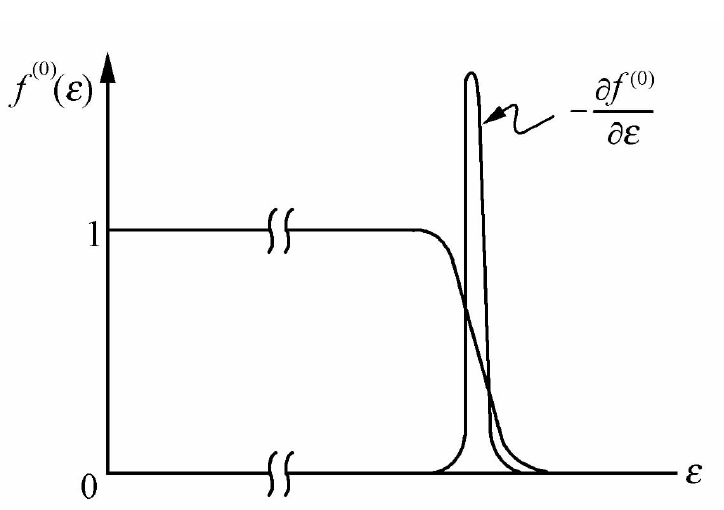
\includegraphics[scale=0.25]{image-20190529174507329.png}
                \caption{费米分布图像}
                \end{figure}
        
        \end{column}
        
        \end{columns}
    
\end{frame}
\subsection{H函数与熵}
\begin{frame}
    \frametitle{H函数与熵}
        H定理和熵增原理看起来似乎有着一样的形式
        是否在H函数与熵中存在某种关系?
        
        
    \begin{block}{}
        事实上,在平衡态下,H函数的确给出了熵。在稀薄气体的前提(也是我们模型的预设)下,有$S\propto(-H+const.)$。 
                                                                                                                                                                                                                                                                                 
    \end{block}
    \begin{block}{}
        为简便起见,取无宏观平动的理想气体($\vec{v}_0=0$),将分布函数代入,H函数:
        \begin{equation*}
            \begin{aligned}
                H&=\iint f\left[\ln n+\frac{3}{2} \ln \left(\frac{m}{2 \pi k T}\right)-\frac{1}{k T} \frac{m \vec{v}^{2}}{2}\right] \mathrm{d}^{3} \vec{v} \mathrm{d}^{3} \vec{r}\\
                &=N\left[\ln \frac{N}{V}+\frac{3}{2} \ln \left(\frac{m}{2 \pi k T}\right)-\frac{3}{2}\right]
            \end{aligned}
        \end{equation*}
        无简并下单原子理想气体熵:
        \begin{equation*}
            S=N k\left[\ln \frac{V}{N}+\frac{3}{2} \ln T+\frac{5}{2}+\frac{3}{2} \ln \left(\frac{2 \pi m k}{h^{2}}\right)\right]
        \end{equation*}
        比较两式,有:
        \begin{equation*}
            S=-k H+C,C=N k\left[1+\ln \left(\frac{m}{h}\right)^{3}\right]
        \end{equation*}

            
        

    \end{block}


        
    

\end{frame}
\section{热寂说}
\subsection{热寂说的简单介绍}
\begin{frame}
    \frametitle{什么是热寂(Heat Death))?为什么?}
    \begin{block}{什么是热寂?}
        \begin{description}
            \item[English]    The heat death of the universe, also known as the Big Chill or Big Freeze, is an idea of an ultimate fate of the universe in which the universe has evolved to a state of no thermodynamic free energy and therefore can no longer sustain processes that increase entropy. Heat death does not imply any particular absolute temperature; it only requires that temperature differences or other processes may no longer be exploited to perform work. In the language of physics, this is when the universe reaches thermodynamic equilibrium (maximum entropy).
            \item[中文] 宇宙的熵会随着时间的流异而增加,由有序向无序,当宇宙的熵达到最大值时,宇宙中的其他有效能量已经全数转化为热能,所有物质温度达到热平衡。这种状态称为热寂。这样的宇宙中再也没有任何可以维持运动或是生命的能量存在。 

        \end{description}
    \end{block}

\end{frame}
    

\begin{frame}
    \frametitle{为什么?}
        热寂说的直接理论依据是热力学第二定律,事实上,热寂说是伴随着热力学第二定律出现而出现的。
        \begin{block}{开尔文勋爵表述}
            \begin{itemize}
                \item “在现今,在物质世界中进行着使机械能散失的普遍趋势……在将要到来的一个有限时期内,除非采取或将采取某些目前世界上已知的并正在遵循的规律所不能接受的措施,否则地球必将开始不适合人类像目前这样居住下去。”
                \item “热力学第二个伟大定律孕含着自然的某种不可逆作用原理,这个原理表明虽然机械能不可灭,却会有一种普遍的耗散趋向,这种耗散在物质的宇宙中会造成热量逐渐增加和扩散,以及势的枯竭。如果宇宙有限并服从现有的定律,那么结果将不可避免地出现宇宙静止和死亡状态。但是,对宇宙中的物质广延设想一个界限是不可能的……”
            \end{itemize}
        
            
        \end{block}
        \begin{block}{克劳修斯表述}
            "The entropy of the universe tends to a maximum."
        \end{block}
    

\end{frame}
\subsection{热寂说的问题与质疑}
\begin{frame}
    \frametitle{有问题吗?}
        热寂说基于热力学第二定律,需要认为:宇宙是有限孤立系统,宇宙能达到平衡态。
        \begin{alertblock}{质疑0:无限系统?}
            \begin{description}
                \item[观点]如果宇宙是无限的,按照熵增原理,体系熵将演化趋于无穷,演化时间也必将趋于无穷,热寂将变成无法企及的平衡态。
                \item[回应]这个质疑没问题,所以我们不考虑宇宙是无限体系的情况。(
            \end{description}
        \end{alertblock}
        \begin{block}{质疑1:宇宙是孤立系统吗?}
            \begin{description}
                \item[观点]现有的观测数据证明,宇宙正在不断膨胀。这样看来,似乎不能用孤立系统描述宇宙。
                \item[回应]暂且不回应是否存在某些机制使得宇宙能够在满足封闭系统的情况下满足实验观测的膨胀。即使宇宙之“外”存在某种结构使得宇宙不构成孤立系统,我们仍可以把这一结构和宇宙放在一起……如此这般,总能找到一个足够大的有限孤立系统,这一系统会达到热寂,而作为子系统的宇宙也必将达到热寂。
            \end{description}
        \end{block}


\end{frame}
\begin{frame}
    \frametitle{有问题吗?}
        \begin{block}{质疑2:统计涨落的存在}
            \begin{description}
                \item[观点]熵增定律是一个统计定律,意味着尽管整个宇宙处在熵减小的状态,但也允许存在有局部的涨落,如人类这样高等生命的出现就是这一涨落的佐证。
                \item[回应]承认涨落的存在,但是足以产生生命的涨落,其概率应该足够小以至于忽略不计。
                \item[回应的回应]我们不是站在这儿吗?
                \item[回应的回应的回应] 
            \end{description}
        \end{block}
        \begin{exampleblock}{质疑3:热力学第二定律有没有问题?}
            \begin{description}
                \item[观点]策梅洛回归性佯谬:孤立的、有限的保守动力学系统在有限的时间内回复到任意接近初始组态的组态(庞加莱回归)。
                \item[回应]庞加莱回归时间是天文数字,哈勃半径内宇宙庞加莱回归时间是$10^{{10}^{{10}^{{10}^{{10}^{{122}}}}}}$,实际意义已经不大,在可以观测的时间内,热力学第二定律是成立的。
                \item[问题来了]对满足遍历性的有限马尔可夫链,一个状态的平均首达时和该状态的平均复现时相等,倘若复现的时间不予考虑,那么涨落说似乎也有些站不住脚。
            \end{description}
        \end{exampleblock}


\end{frame}
\begin{frame}
    \frametitle{有问题吗?}
    \begin{exampleblock}{质疑4:麦克斯韦妖}
        麦克斯韦妖对于热寂说的诘难来自于对熵增加原理的质疑,之前的讨论班报告中已经有过了详尽的论述。
    \end{exampleblock}
    
        \begin{block}{质疑5:引力系统的负热容性}
            \begin{description}
                \item[观点]引力系统有“负热容”性,即动能的增大需要引力势能的减小。这样的系统是无法达到热平衡的。
                \item[回应]既然无法达到平衡态,热容定义所需要的温度又应该如何定义?定义出的温度和动能的关系是否还可以满足?
            \end{description}
        \end{block}
        
        
       


\end{frame}



\end{document}
